       
 
 
\chapter{Calibration procedure}
\label{chapter:calibration}

%\section{Review of level0 data}
%The thermal and electrical environment of a satellite may cause
%receiver instabilities, which must be compensated. Whereas ground
%based systems may have relatively stable gain but changing system
%temperature due to unstable weather conditions, the Odin satellite
%shows the opposite behaviour: stable noise figures in spite of cyclic
%gain variations during one orbit.

%\section{Measurement sequence and radiance calibration process}


\section{Processing pipeline}

Raw science and house-keeping data are downloaded at
Esrange and transferred to a data archive housed by the Parallel
Data Centre (PDC) at the Royal Institute of Technology (KTH)
in Stockholm. The data processing for the calibration \smr\
measurements are performed at the Dept. of Earth and Space
Sciences at Chalmers University of Technology (Chalmers) in Gothenburg.
A file system at Chalmers is synchronized with the Level0-file archive 
at KTH. The KTH archive also contains files with reconstructed attitude
information.  Science and house-keeping data within those files
are imported into Level0 tables of an Odin calibration database
(a postgresql database). 
Dedicated algorithms to process and combine new Level0 to Level1B
data are executed on a regular basis and are described in this
chapter. Level1B data are stored in tables of the Odin calibration database.  
Chapter 3 describes the its format and how to access the Level1B data.
%\lcomment{BR}{should this be included?}



%\section{Important aspects for calibration}%
%
%\lcomment{BR}{skip this section}
%
%The definition of a scan (in calibration version 8) is based
%on the measurement sequence. A scan consists of all type of signals and data that
%where recorded from the first 'load signal' (when such are collected) until the
%next sequence of 'load signals'. In practise, this is equivalent to all 
%measurements collected between the lower turning point and upper turning point
%(or vice versa) of the limb-scanning motion.
%
%An important aspect for the calibration is to take into account
%that the main beam signal is always at a higher level than the cold sky signal,
%due to thermal emission from a baffle, that only affect the main beam signal.
%
%It has also turned out out that a slight imbalance between signal and 
%reference phase introduces instabilities seen as low-level ripple 
%in calibrated atmospheric spectra, if not taken into account. %
%
%frequency calibration%
%
%pointing?
%the spectrometer passbands. This ripple is stable in the IF band,
%and can be measured towards a blank region of the sky and subsequently
%be subtracted from target spectra.
%A scan is then defined as all measurements collected between two hot
%load signals, which in practise is equivalent to all measurements
%collected between the lower turning point and upper turning point
%(or vice versa) of the limb-scanning motion. Table 2
%lists the scanning range of the three main scanning modes used.




\section{Radiometric calibration algorithm}

\subsection{Auto-correlator data}

Data from the ACs must be transformed to spectra in the frequency domain
prior to the radiometric calibration.
This preparation of AC data basically involves a quantisation correction and the application
of a Fourier transform.
In the spectrometer hardware, the input signal is quantized into three levels: 
high positive, high negative, and low amplitude. The input signal is furthermore delayed, 
cross multiplied and integrated to obtain a measure of the auto-correlation function of the 
input signal \(s(t)\). 

\begin{itemize}

\item Accurate quantization correction requires accurate knowledge of the threshold
 levels used at quantization. The quantization correction used is only valid 
if the absolute values of the the positive and negative threshold levels are equal. 
The \smr\ correlators provide monitor channels to check the
assumption of equal absolute values of the positive and negative threshold levels.
Only when this condition is fulfilled the data will be further processed.

\item The estimation of the true correlation \(\rho\) from the measured correlation
coefficient \(r\) at lag \(\tau\) is then achieved by performing a quantization correction using
Kulkarni and Heiles approximation described in \citet{ohlberg:theod:03}.

\item a Hanning smoothing is applied, which gives that the obtained resolution 
of the spectra is 2\,MHz although the channel spacing is 1\,MHz

\item The Fourier transform of the auto correlation function gives the
power spectral density, or a spectrum in the frequency domain.


\end{itemize}


\subsection{Radiances}


The radiance emitted by a blackbody per frequency unit is
\begin{equation}
 B_{\nu} = \frac{2h\nu^{3}}{c^{2}}\frac{1}{\exp(\frac{h\nu}{kT})-1},
\end{equation}   
where \(\nu\) is frequency, \(h\) is Planck's constant, \(k\) is Boltzmann's constant,
\(c\) is the speed of light, and \(T\) is the physical temperature of the
blackbody.
The Rayleigh--Jeans correspondence (valid when \(h\nu/kT\)<<1) reads
\begin{equation}
 B_{v}=\frac{2\nu^{2}kT}{c^{2}}.
\end{equation}

The \smr\ radiometers are heterodyne systems which receive a power (\(P_{\nu}\))
per unit frequency range (spectral power density),
\begin{equation}
P_{\nu} = \frac{c^{2}}{2\nu^{2}}B_{\nu}
\end{equation} 
where \(\nu\) is frequency, \(h\) is Planck's constant, \(k\) is Boltzmann's constant,
when viewing a blackbody source at temperature (\(T\)) that completely
fills the antenna field of view. 
If the Rayleigh--Jeans approximation is valid, we then have that
\begin{equation}
P_{\nu} = kT.
\end{equation}
For a theoretical receiver and channel of bandwidth \(\Delta \nu\), with zero loss and gain 
and a unit frequency response, the received power is
\begin{equation}
 P = kT\Delta \nu.
\end{equation}   

Brightness temperature (\(T_{b}\)) and antenna temperature (\(T_{a}\))
are two closely related quantities. They are both defined with respect to a 
matching blackbody temperature. However, they differ in that \(T_{b}\) corresponds 
to radiance while \(T_{a}\) must be seen as a measure on power.
The brightness temperature is defined as the physical temperature 
a blackbody would have to generate the same radiance as the one of concern.
That is, for a given radiance \(I\), \(T_{b}\) is defined as
\begin{equation}
 I = B_{v}(T_{b}),
\end{equation}
and in the Rayleigh--Jeans approximation this gives
\begin{equation}
 T_{b} = \frac{c^{2}I}{2kv^{2}},
\end{equation}
and the Rayleigh--Jeans temperature of a blackbody can be written as 
\begin{equation}
 T_{b} = \frac{h\nu}{k}\frac{1}{\exp(\frac{h\nu}{kT})-1}.  
\end{equation}


The antenna temperature is defined as the temperature of an ideal black
body that would result in the same received power at the antenna aperture 
as in the actual case, which gives that (using Rayleigh--Jeans approximation)
\begin{equation}
T_{a} = \frac{P}{k\Delta \nu}
\end{equation}

A radiometer detects radiant power and the calibration is most 
easily discussed in terms of input power. As will be shown below, 
the measured power can be converted to an
antenna or brightness temperature or a radiance, but it should be 
remembered that it is only power that can actually be measured.


\subsection{\smr\ observation sequence and measured signals} 
\label{sec:smrobs}

\begin{figure}[t]
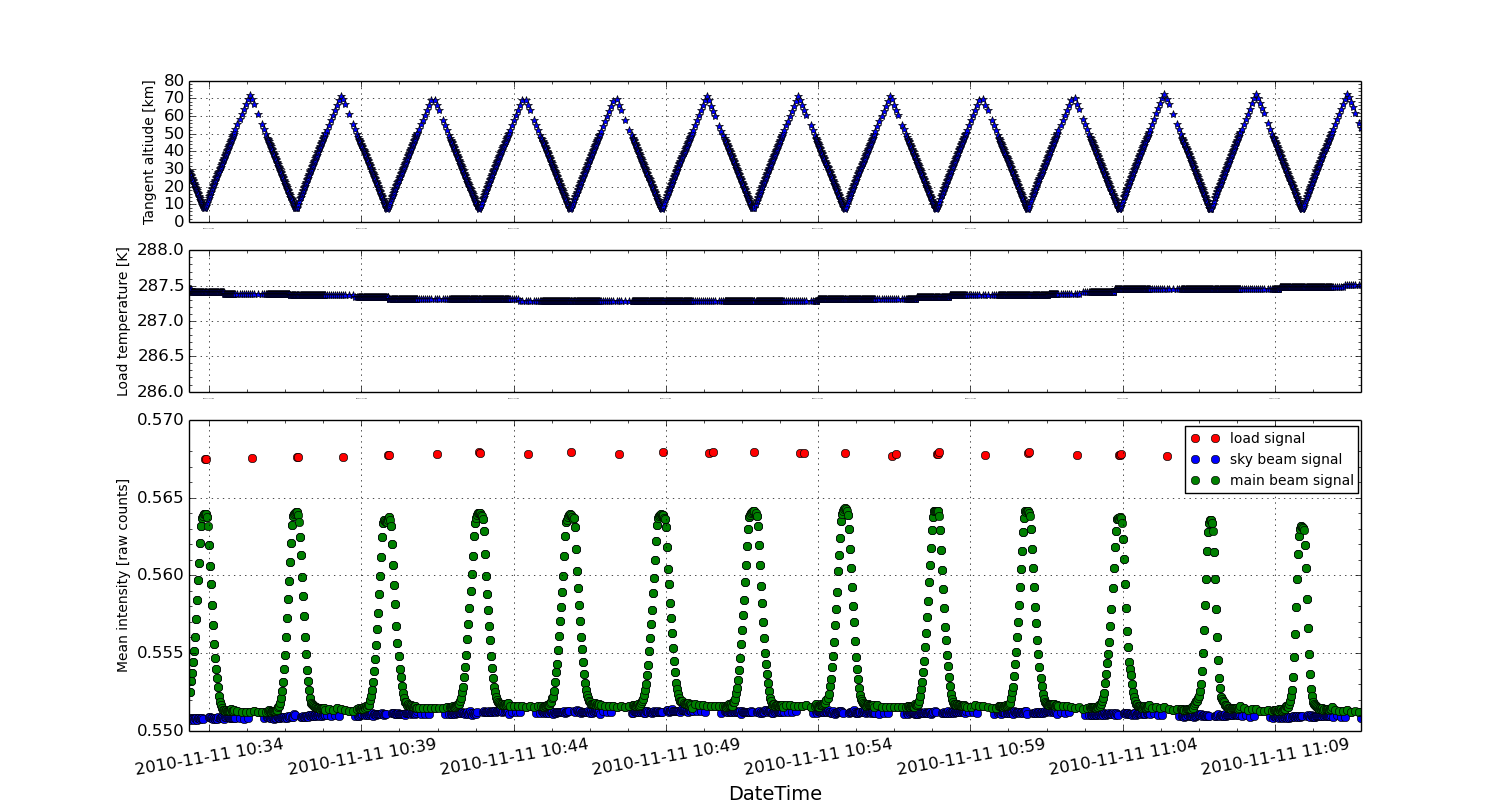
\includegraphics[width=14cm]{cal_signals.png}
\caption{ Intensity variation of one of the sub-bands of freqmode~1
during a number of scans for the three types of signals involved
in the intensity calibration scheme.}
\label{fig:intensityvar}
\end{figure}



For calibration purposes, Odin/SMR performs areonomy observation in a switching
mode, i.e. switching between the main beam and an unfocused sky beam. 
In nominal operation every other recorded signal comes from an unfocused cold sky
beam, except around the lower and upper turning points of the scan where the reference
beam is directed towards the internal load (typically three consecutive load spectra are
recorded). The load acts as a blackbody emitter at an ambient temperature of around 285
K. 

The intensity calibration of \smr\ is thus performed by using
information from three types of signals (see Fig~\ref{fig:intensityvar}), 
i.e. the sky beam signal (\(c_{s}\)), the load signal (\(c_{l}\)), 
and the main beam signal (\(c_{a}\)).
The calibration scheme is based on the assumption that the
digital value (e.g. \(c_{a,i}\)) read out from channel \(i\) of the
spectrometer is proportional to the power of the
observed signal. The contributions to the three signals
can be expressed as:

\begin{equation}
c_{a,i}=g_{i}\left(\eta_{a} T_{a,i} + T_{rec,i} + (1-\eta_{a})T_{amb,i} \right) = 
g_{i}\left(\eta_{a} T_{a,i} + T_{rec,i} + T_{sp} \right) ,
\end{equation}
\begin{equation}
\label{eq:skybeam}
c_{s,i}=g_{i}\left(T_{s,i}+T_{rec,i}\right) \approx g_{i}\left(T_{rec,i}\right),
\end{equation}
\begin{equation}
c_{l,i}=g_{i}\left(T_{l,i}+T_{rec,i}\right),
\end{equation}
where \(g_{i}\) is the receiver gain, \(\eta_{a}\) is the main beam
efficiency (it is assumed that beam efficiencies for
both the sky beam and load signals are unity),
\(T_{amb,i}\) is the receiver ambient temperature,
and \(T_{rec,i}\) is the receiver noise temperature.
\(T_{a,i}\), \(T_{s,i}\), and \(T_{l,i}\) are the antenna temperature,
cosmic background temperature, and load temperature all expressed
as equivalent Rayleigh--Jeans brightness temperatures (\(T_{b}\)).
The Rayleigh--Jeans brightness temperature of the cosmic background radiation
at 500 GHz is only 0.003\,K, and typical \(T_{rec}\) value of \smr\ is 3000\,K,
thus the approximation in eq.~\ref{eq:skybeam} results in negligible error.

The main beam signal is always at a higher level than the cold sky signal
(Fig.~\ref{fig:intensityvar}), which is due 
to thermal emission from a baffle which only affects the main beam signal.
Thus, the main beam intercepts with the baffle
and the spill over contribution (\(T_{sp}\)):
\begin{equation}
\label{eq:tspill1}
T_{sp}=(1-\eta_{a})T_{amb}.
\end{equation}

\subsection{Calibration: basic equations}
\label{sec:caleq}
The aim of the calibration process is to use  
information from the signals described in Sect.~\ref{sec:smrobs}
in order to derive an estimate of the antenna temperature.
Here we derive expressions for how the unknown \(T_{rec,i}\),
\(g_{i}\), \(T_{sp}\), \(n_{a}\), and \(T_{a,i}\) can be derived.
In Sect.~\ref{sec:calscheme} the actual \smr\ calibration is described. 

Eq.~\ref{eq:skybeam} gives that
\begin{equation}
\label{eq:trec}
T_{rec,i}=\frac{c_{s,i}}{g_{i}},
\end{equation}
and \(g_{i}\) can be obtained from the difference between \(c_{l,i}\) and
 \(c_{s,i}\), i.e.
\begin{equation}
\label{eq:gain}
g_{i}=\frac{c_{l,i}-c_{s,i}}{T_{l,i}-T_{s,i}}.
\end{equation}
By combining Eq.~\ref{eq:trec} and~\ref{eq:gain} we obtain
\begin{equation}
\label{eq:trec2}
T_{rec,i}=c_{s,i}\frac{{T_{l,i}-T_{s,i}}}{c_{l,i}-c_{s,i}}.
\end{equation}

\(T_{a,i}\) can be obtained from the difference between between
\(c_{a,i}\) and \(c_{s,i}\), i.e.
\begin{eqnarray}
\label{eq:ta}
T_{a,i} &=& \frac{1}{\eta_{a}}\left(\frac{c_{a,i}-c_{s,i}}{g_{i}} - T_{sp}\right) \nonumber\\
 &=& \frac{1}{\eta_{a}}\left( \left(c_{a,i} - c_{s,i}\right)\frac{T_{rec,i}}{c_{s,i}} -T_{sp} \right). 
\end{eqnarray}

For measurements at tangent altitude above the atmosphere
\(T_{a,i}\) = 0. Thus, we have that for these measurements
to a very good approximation

\begin{equation}
\label{eq:tspill2}
T_{sp,i}= \left(c_{a,i}-c_{s,i}\right)\frac{T_{rec,i}}{c_{s,i}}.
\end{equation}

Combining Eq.~\ref{eq:tspill1} and~\ref{eq:tspill2} gives that
\begin{equation}
\label{eq:eta}
\eta_{a}=1-\frac{T_{sp}}{T_{amb}}=1-\frac{\left(c_{a,i}-c_{s,i}\right)\frac{T_{rec,i}}{c_{s,i}}}{T_{amb}}.
\end{equation}

\subsection{Low level ripple}
\label{sec:ripples}
Equation~\ref{eq:ta} can be thought of as the main intensity
calibration equation for the \smr\ calibration scheme.
In the derivation of Eq.~\ref{eq:ta}
the reference signals are assumed to be ``clean''.
In practice, there seems to be a small imbalance between 
measurements and references for \smr. 
Small perturbations of the sky and load signals will
result in undesired features in calibrated
spectra (which we denote as ``ripple'') 
if not taken into account (see Fig.~\ref{fig:ripple1}).
%This section describes how 
%ripple on those signals
%can be taking into account in the calibration process.
The sensitivity of calibrated \(T_{a,i}\) 
to small perturbations on \(T_{s,i}\) and \(T_{l,i}\) are:
\begin{equation}
\frac{dT_{a,i}}{dT_{s,i}}=\frac{1}{\eta_{a}}\left(1-\frac{c_{a,i}-c_{s,i}}{c_{l,i}-c_{s,i}}\right)\approx \frac{1}{\eta_{a}}\left(1-\frac{T_{a,i}}{T_{l,i}}\right)
\end{equation}
and
\begin{equation}
\frac{dT_{a,i}}{dT_{l,i}}=\frac{1}{\eta_{a}}\left(\frac{c_{a,i}-c_{s,i}}{c_{l,i}-c_{s,i}}\right)\approx \frac{1}{\eta_{a}}\left(\frac{T_{a,i}}{T_{l,i}}\right).
\end{equation}
Thus, the sensitivity is linearly proportional to \(T_{a,i}\).
When \(T_{a,i}\) is close to or 0 K (as it is for measurements at high
tangent altitudes) the sensitivity to perturbations of
the sky beam signal is at its maximum.
On the other hand, perturbations on the load signal then have practically
no impact on \(T_{a,i}\).
If \(T_{a,i}\) were equal to the load temperature the situation would be reversed,
though this is never the case in practice.

A model for the removal of the effects of ripple on the reference signals
on estimated \(T_{a,i}\) (from Eq.~\ref{eq:ta}) to achieve a new
better estimate \(T^{'}_{a,i}\) of the antenna temperature then reads
\begin{equation}
\label{correction}
T^{'}_{a,i}=T_{a,i}-\frac{1}{\eta_{a}}\left(1-\frac{T_{a,i}}{T_{l,i}}\right) s_{0,i}-
 \frac{1}{\eta_{a}}\left(\frac{T_{a,i}}{T_{l,i}}\right) s_{1,i},
\end{equation}
where \(s_{0,i}\) and \(s_{1,i}\) can be seen as spectra that contain
the ripple induced features for \(T_{a,i}\)=0\,K and \(T_{a,i}\)=\emph{load~temperature}
respectively.

\subsection{Intensity calibration scheme} 
\label{sec:calscheme}

The intensity calibration scheme can be divided into two parts. The first part can be
seen as a scan based calibration scheme, in which the Equations of Sect.~\ref{sec:caleq} are applied.
The second part takes ripples (\ref{sec:ripples}) into account and uses the results
(for a long period of time of measurements) from the first part of the calibration.


\subsection*{Part 1}

The Odin calibration scheme (version 8) is scan-based, as will be described below, and
this is one of the main differences to previous verisons. 

Equation~\ref{eq:ta} is the key equation of the calibration.
From this equation we see that to calibrate a given target signal
we need to determine \(T_{rec,i}\), \(T_{sp}\), \(\eta_{a}\),
and \(c_{s,i}\). Some of these variables, i.e. \(T_{rec,i}\), \(T_{sp}\), and \(\eta_{a}\)
are assumed to be fairly stable over short time scales.
Common values of all these parameters are used for
the calibration of all \(c_{a}\) signals within a given scan.
\(g\) can vary significant over short time-scales,
and this is taken into account by the division of \(c_{a}\) with
\(c_{s}\) (with a unique \(c_{s}\) for each \(c_{a}\)
signal of the scan). The intensity calibration scheme (version 8)
for a given scan can be summarized as:
\begin{itemize}
\item collect all relevant level0 and level1 data for the scan and for an
additional time-period of \(\pm\)45 minutes.
It is assured that only data with ssb attenuator settings
as in the first load signal of the scan is used.
Furthermore, only data where calibrated sky frequencies changes by less
than 1 MHz from one signal to another is used.

\item filter data, i.e. remove untrusted reference signals:\newline
Only sky beam signals from Sky Beam 1 (SK1) are used.
An SK1 signal is only used if the previous
reference signal was from SK1.
SK1 signals with skybeamhit flags EARTH1, MOON1, and SUN1 are not used.
Only the second load signal is used for each sequence of load signals
observation.

\item estimate an average \(T_{rec}\) spectrum:\newline
Equation~\ref{eq:trec2} is applied to calculate \(T_{rec}\)
for all kept \(c_{l}\) signals, where
the two nearest \(c_{s}\) signals are linearly interpolated
in time to \(c_{l}\).
The mean value of all \(T_{rec}\) is used as the
common \(T_{rec}\) spectrum within a given scan.
\item estimation of a scalar \(T_{sp}\):\newline
\(T_{sp}\) is estimated from measurements at high tangent altitude
by applying Eq.~\ref{eq:tspill2}.
The median of the median
from all \(c_{a}\) signals, measured within the top 10 km
of the range of tangent altitudes, is used as a common scalar \(T_{sp}\).
\item estimation of \(\eta_{a}\):\newline
\(\eta_{a}\) is estimated by applying Eq.~\ref{eq:eta},
using the estimated \(T_{sp}\) described above, and an
assumed \(T_{amb}\) of 300 K.
\item estimate \(T_{a}\): \newline
apply Eq.~\ref{eq:ta}, using the estimated parameters as described
above and
the two nearest \(c_{s}\) signals are linearly interpolated
in time to \(c_{a}\).
\end{itemize}



\subsection*{Part 2}

\begin{figure}[t]
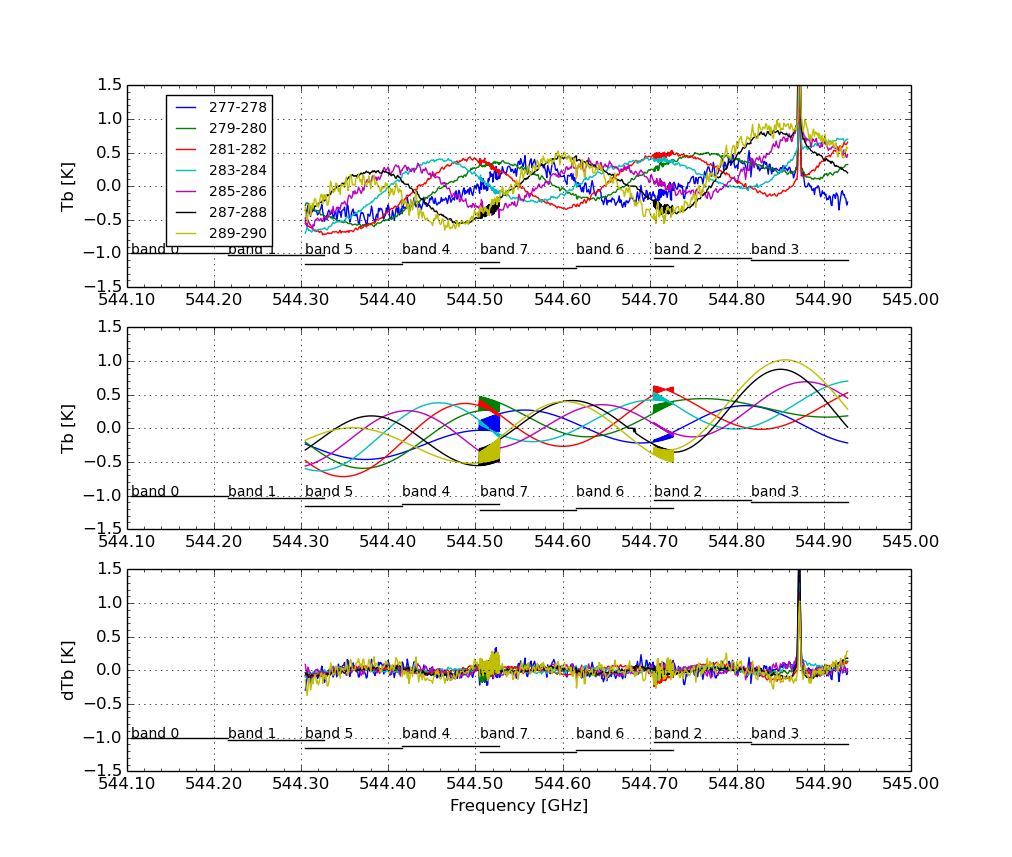
\includegraphics[width=14cm]{calibration_step2_fig.png}
\caption{Schematic of part 2 of the intensity calibration.
The upper panel shows uncorrected average spectra for frequency mode 2 observations
with tangent points between 80 and 120\,km. The color-coding corresponds
to ambient temperature of the satellite (hotload temperature).
The middle panel shows fits of the ripple of the spectra in the 
upper panel. The lower panel shows the residual.}
\label{fig:ripple1}
\end{figure}



Part 2 of the calibration deals with the removal
of the effects of ripple on the sky signal on calibrated
spectra from part 1, which neglects this effect.
The removal of the artifacts introduced by the sky signal
ripple is a fairly straight-forward task, as the artifacts
can be estimated from high tangent point measurements
where we know that the intensity of a calibrated spectrum should be 0 K.

Ripple on the load signal is more complicated from
a calibration perspective. The artifacts, in calibrated
atmospheric spectra, from ripple on the
load signal can be seen as weak signal on top of a strong
atmospheric signal, and thus not easy to detect.
For this reason, we leave this effect unresolved.

Figure~\ref{fig:ripple1} shows median spectra of calibrated (Part 1) spectra
from measurements at high tangent altitudes for one of the
observation mode of AC1 (for the further discussion on this figure
ignore the left-most part of the spectra, which comes from two 
problematic bands of AC1 that should not be used). 
These spectra are expected to be 
centered around 0~K (except for the ozone line between 544.8--544.9~GHz), 
but due to ripple in the sky signal we can see a wave pattern in the spectra.
Figure~\ref{fig:ripple1} also indicates that the phase of the wave pattern
depends on the measurement conditions, and the temperature of
the load (ambient temperature) is used in Fig~\ref{fig:ripple1}
to describe the measurement condition.


The calibration scheme (Part 2) is as follows:
\begin{itemize}
\item Extract median spectra of calibrated spectra 
(from Part 1:ac\underline{ }level1b table) 
from measurements at tangent altitudes above 80 km for a range of hot load 
temperatures ([277--278~K, 278--279~K, ..., 289--290~K]) 
for each observation mode, and import the spectra
into the ac\underline{ }level1b\underline{ }average table
%(Table~\ref{table:ac1c1})
\item Estimate a fit to the median spectrum for each mode by
\begin{enumerate}
\item applying a filter that removes channels which are contaminated by 
atmospheric information or lines from the median spectrum 
\item using the target fitting function  
\begin{equation}
y=a+ b\sin(cf+d)
\end{equation}
where \(f\) is the frequency and \(a,b,c,d\) parameters to estimate,
in order to fit the spectrum for each of the four modules of AC1 or AC2.
The fitting is performed in such a way that \(c\) is forced 
to be equal for all of the four modules. 
Import the fit into the ac\underline{ }cal\underline{ }level1c
table
%(Table~\ref{table:ac1b2})
\end{enumerate}
\item Apply the correction.\\
Equation~\ref{correction} is applied to correct a given calibrated 
spectrum (from part~1), where the fit of the median spectrum
with matching hot load temperature range is used as the \(s_{0}\)
spectrum. 
%This is done within the program/functions, described in
%Sect.~\ref{sec:officialexport}, used to export the official
%level1b-product.  
\end{itemize}



\section{Radiometric performance and uncertainties}
\label{sec:radper}


\begin{table}
\caption{ Average \(T_{rec}\), \(T_{sp}\), and radiometric noise (for 1.8 sec. integration time) for the various frequency modes }
\label{table:config5}
\begin{tabular}{|l|l|l|l|l|l|l|}
  \hline
  \textbf{Backend} & \textbf{Frontend} & \textbf{LO freq {[}GHz{]}} & \textbf{FM} & \textbf{\(T_{rec}\) {[}K{]}} & \textbf{\(T_{sp}\) {[}K{]}} & \textbf{\(\Delta T [K]\)} \\
  \hline
  AC1              & 495 A2            & 492.750                    & 23          & 3000                  & 7.0  & 2.0\\
  \cline{3-3}
  \cline{4-4}
  \cline{5-5}
  \cline{6-6}
  \cline{7-7}
                   &                    & 499.698                   & 25          & 3500 *                & 6.2  & -\\
  \cline{2-2}
  \cline{3-3}
  \cline{4-4}
  \cline{5-5}
  \cline{6-6}
  \cline{7-7}
                   & 549 A1             & 548.502                  & 2            & 2800 *                & 8.0 & 1.8 \\
  \cline{3-3}
  \cline{4-4}
  \cline{5-5}
  \cline{6-6}
  \cline{7-7}
                  &                     & 553.050                  & 19           & 2900 *                & 7.3 & 1.9 \\
  \cline{3-3}
  \cline{4-4}
  \cline{5-5}
  \cline{6-6}
  \cline{7-7}
                  &                     & 547.752                  & 21           & 3100 *                & 8.6 & 2.0 \\
  \cline{3-3}
  \cline{4-4}
  \cline{5-5}
  \cline{6-6}
  \cline{7-7}
                  &                     & 553.302                  & 23           & 3200                  & 6.8 & 2.1 \\
  \cline{2-2}
  \cline{3-3}
  \cline{4-4}
  \cline{5-5}
  \cline{6-6}
  \cline{7-7}
                 & 555 B2              & 553.298                   & 13           & 3200                  & 14.0 & 2.1 \\
  \cline{2-2}
  \cline{3-3}
  \cline{4-4}
  \cline{5-5}
  \cline{6-6}
  \cline{7-7}
                & 572 B1               & 572.762                   & 24           & 3200 *                & 9.4 & 2.1 \\
  \hline
  AC2           & 495 A2               & 497.880                   & 1            & 3200                  & 6.1 & 2.1\\
  \cline{3-3}
  \cline{4-4}
  \cline{5-5}
  \cline{6-6}
  \cline{7-7}
                &                      & 492.750                   & 8            & 3200                  & 7.4 & 2.1\\
  \cline{3-3}
  \cline{4-4}
  \cline{5-5}
  \cline{6-6}
  \cline{7-7}
                &                      & 494.750                   & 17           & 3200                  & 6.7 & 2.1\\
  \cline{3-3}
  \cline{4-4}
  \cline{5-5}
  \cline{6-6}
  \cline{7-7}
                &                      & 499.698                   & 25           & 3200                 & 7.6 & 2.1\\
  \cline{2-2}
  \cline{3-3}
  \cline{4-4}
  \cline{5-5}
  \cline{6-6}
  \cline{7-7}
                & 572 B1              & 572.762                    & 14           & 3700 *              & 9.9 & 2.4\\
  \cline{3-3}
  \cline{4-4}
  \cline{5-5}
  \cline{6-6}
  \cline{7-7}
                &                     & 572.964                    & 22           & 3700 *              & 10.0 & 2.4\\
  \hline
\end{tabular}
\end{table}

In this section we deal with uncertainties that are related to calibrated \smr\ spectra. 
In Sect.~\ref{sec:radnoise} we describe uncertainties related to radiometric noise.
In Sect.~\ref{sec:gainvar} we describe uncertainties related to rapid gain fluctuations.
In Sect.~\ref{sec:otheruncer} we describe uncertatinties that are related to imperfect knowledge
of load temperature and main beam efficiency.
In Sect.~\ref{sec:trends} trend uncertainties are explored.
In Sect.~\ref{notesoncorr} we describe the noise correlations. 
In Sect.~\ref{sec:caluncer} we describe the noise estimate output from the calibration routine.  


\subsection{Uncertainties related to radiometric noise}
\label{sec:radnoise}

In the \smr\ calibration process three types of signals are used (all of them containing radiometric noise)
and the obtained noise in calibrated spectra is sensitive to noise in
all of these measurements. 
The noise contribution can be divided into three terms
(1) the radiometer noise contribution,
(2) interpolated reference noise contribution, and (3) interpolated gain noise contribution
\cite{jarnot:04}.

These contributions (derived in the following sub-sections) gives that the noise on an individual channel \(\Delta T_{i}\) of a 
calibrated \smr\ spectrum using the calibration scheme described in Sect.~\ref{sec:calscheme}. 
The noise can be described by
\begin{equation}
\Delta T_{i}^{2} =  \frac{1}{B\tau} \left( (T_{rec,i}+T_{a,i})^2 + \frac{T_{rec,i}^2}{2} +
   \frac{T_{a,i}^{2}}{n} \left( \left( \frac{T_{rec,i} + T_{l,i}}{T_{l,i}} \right)^2 + 
   \left( \frac{T_{rec,i} }{T_{l,i}} \right)^2 \right) \right).
\label{eq:raderror}
\end{equation}
For measurements with a nearly blank background (i.e. \(T_{a,i}\approx\)0), uncertainties in the gain estimate 
have low impact and the noise expression reduces to
\begin{equation}
\Delta T_{i} =  T_{rec,i}\sqrt{\frac{3}{2}\frac{1}{B\tau}}.
\label{eq:higaltnoise}
\end{equation}
In Table~\ref{table:config5} typical \(T_{rec}\) values and radiometric noise levels
(for measurements having high tangent points)
of the main frequency modes of \smr\ are listed.


%The noise on an individual channel, \(\Delta T\) , is commonly represented by
%\begin{equation}
%\Delta T = T_{sys}\sqrt{ \frac{1}{B\tau} + \left( \frac{\Delta g}{g} \right)^2 }
%\label{eq:prec}
%\end{equation}
%where \(T_{sys}\) is the combination of receiver system temperature (\(T_{rec}\)) and
%scene radiance (\(T_{a}\)), \(B\) is the channel bandwidth,
%\(\tau\) is the integration time of each measurement, and \(\frac{\Delta g}{g}\)
%is a gain variation term. The \(\frac{1}{B\tau}\) component is commonly referred to as
%radiometer noise, and is uncorrelated between channels.
%The gain variation term is more likely to be correlated between channels.
%quation~\ref{eq:prec} is not complete for \smr\ as it ignores the noise
%coming from noise on interpolated reference measurements.
%We here derive a more complete expression:

As a starting point to derive Eq.~\ref{eq:raderror} we take the derivative of \(T_{a,i}\) 
with respect to \(c_{a,i}\), \(c_{s,i}\), and \(g_{i}\):

\begin{equation}
\frac{\partial T_{a,i}}{\partial c_{a,i}} \approx \frac{1}{g_i}, 
%\implies \Delta T_{a,i}^{2}=\frac{\Delta c_{a,i}^{2}}{g_{i}^2}
\end{equation}

\begin{equation}
\frac{\partial T_{a,i}}{\partial c_{s,i}} \approx \frac{1}{g_i}, 
%\implies \Delta T_{a,i}^{2}=\frac{\Delta c_{s,i}^{2}}{g_{i}^2}
\end{equation}

\begin{equation}
\frac{\partial T_{a,i}}{\partial g_{i}} \approx -\frac{c_{a,i}-c_{s,i}}{g_{i}^{2}} \approx \frac{T_{a,i}}{g_i}, 
%\implies \Delta T_{a,i}^{2}=T_{a,i}^{2}\frac{\Delta g_{i}^{2}}{g_{i}^2}
\end{equation}
which implies:

\begin{equation}
\Delta T_{i}^{2} = \frac{\Delta c_{a,i}^{2}}{g_{i}^2} + \frac{\Delta c_{s,i}^{2}}{g_{i}^2} + T_{a,i}^{2}\frac{\Delta g_{i}^{2}}{g_{i}^2},
\end{equation}
where the terms on the right hand side is (1) the radiometer noise contribution,
(2) interpolated reference noise contribution, and (3) interpolated gain noise contribution.  
In the following sections these terms are described in more detail.

\subsection*{Precision: radiometer noise contribution}
The radiometer noise contribution induced noise variance in calibrated \(T_{a,i}\) is simply
\begin{equation}
\frac{\Delta c_{a,i}^{2}}{g_{i}^2} = \frac{T_{sys}^{2}}{B\tau}.
\end{equation}

%It should be noted that this noise is not uncorrelated between neighbouring channels
%in \smr\ spectra, as a Hanning smoothing is applied in the calibration process
%(noise is effectively reduced as this can be seen as an increase in bandwidth).    


\subsection*{Precision: interpolated reference noise contribution}
In the \smr\ calibration scheme, and for the nominal situation, the sky beam interpolated
reference signal can be written
\begin{equation}
\hat{c}_{s,i}(t_{j+1}) = \frac{1}{2}c_{s,i}(t_{j}) + \frac{1}{2}c_{s,i}(t_{j+2}), 
\end{equation}
where \(t_{j}\) represent time.  
If the gain fluctuations are small or follow a linear variation during the
observation sequence, the noise in \(\hat{c}_{s,i}(t_{j+1})\) is only due to radiometric
noise and induced noise variance in calibrated \(T_{a,i}\) is
\begin{equation}
\frac{\Delta c_{s,i}^{2}}{g_{i}^2} = \frac{T_{rec}^{2}}{2B\tau}.
\end{equation}

In practice there is also a finite error due to non-linear and non-captured
gain variation and this is described in Sect~\ref{sec:gainvar}.

   
\subsection*{Precision: interpolated gain noise contribution}

In the calibration scheme, the gain is estimated as
\begin{equation}
g_{i}(t_{j+k}) = \frac{\hat{c}_{s,i}(t_{j+k})}{\overline{T}_{rec,i}} = \hat{c}_{s,i}(t_{j+k})\left(\frac{1}{n}\sum_{j=1}^{n}T_{rec,i}(t_{j})\right)^{-1}, 
\end{equation}
where
\begin{equation}
T_{rec,i}(t_{j}) = \hat{c}_{s,i}(t_{j}) \frac{ T_{l} - T_{s} }{  c_{l,i}(t_{j})- \hat{c}_{s,i}(t_{j})  }.
\end{equation}
That is, the precision of the interpolated gain depends on the precision of an interpolated
reference measurement and on an average \(T_{rec}\). 

We first note that
\begin{equation}
\frac{\partial g_{i}}{\partial \hat{c}_{s,i}(t_{j+k})} = \frac{1}{\overline{T}_{rec,i}}
\end{equation}

\begin{equation}
\frac{\partial g_{i}}{\partial T_{rec,i}} = - \frac{\hat{c}_{s,i}(t_{j+k})}{\overline{T}_{rec,i}^2}.
\end{equation}

For an individual \(T_{rec}\) estimate, we have that
\begin{equation}
 \frac{\partial T_{rec,i}}{\partial c_{s,i}(t_{j})} = \frac{(T_{l}-T_{s})(c_{l,i}-c_{s,i}) + c_{s,i}(T_{l}-T_{s})}
{(c_{l,i}-c_{s,i})^2} \approx \frac{T_{rec,i}}{g_{i}T_{l}}
\end{equation}

\begin{equation}
 \frac{\partial T_{rec,i}}{\partial c_{l,i}} = \frac{-c_{s,i}(T_{l}-T_{s})}{(c_{l,i}-c_{s,i})^2} \approx -\frac{T_{rec,i}}{g_{i}T_{l}}
\end{equation}
Thus, we have

\begin{equation}
 \frac{\partial g_{i}}{\partial c_{l,i}} = \frac{\partial g_{i}}{\partial T_{rec,i}}\frac{\partial T_{rec_{i}}}{\partial c_{l,i}}=
\frac{1}{T_{l,i}-T_{s,i}} 
%\implies \Delta g_{i}^{2} =  \frac{\Delta c_{l,i}^{2}}{(T_{l,i}-T_{s,i})^2}
\end{equation}

\begin{equation}
 \frac{\partial g_{i}}{\partial c_{s,i}} = \frac{\partial g_{i}}{\partial T_{rec,i}}\frac{\partial T_{rec_{i}}}{\partial c_{s,i}} =
\frac{-1}{T_{l,i}-T_{s,i}} 
%\implies \Delta g_{i}^{2} =  \frac{\Delta c_{s,i}^{2}}{(T_{l,i}-T_{s,i})^2}
\end{equation}
which implies:

\begin{equation}
\Delta g_{i}^{2} =  \frac{\Delta c_{l,i}^{2} + \Delta c_{s,i}^{2}}{(T_{l,i}-T_{s,i})^2} + \frac{ \Delta c_{i}^{2}(t_{j+1})}{T_{rec,i}^{2}}
\approx \frac{\Delta c_{l,i}^{2} + \Delta c_{s,i}^{2}}{T_{l,i}^2}
\end{equation}
and

\begin{equation}
T_{a,i}^{2}\frac{\Delta g_{i}^{2}}{g_{i}^2} = \frac{T_{a,i}^{2}}{T_{l,i}^2} \frac{\Delta c_{l,i}^{2} + \Delta c_{s,i}^{2}}{g_{i}^{2}},
\end{equation}
or, if we take into account that \(T_{rec}\) spectrum is an average from \(n\) measurements

\begin{equation}
 T_{a,i}^{2}\frac{\Delta g_{i}^{2}}{g_{i}^2} =  \frac{1}{B\tau} \left(
   \frac{T_{a,i}^{2}}{n} \left( \left( \frac{T_{rec,i} + T_{l,i}}{T_{l,i}} \right)^2 + \left( \frac{T_{rec,i} }{T_{l,i}} \right)^2 \right) \right).
\end{equation}


%\begin{equation}
%\frac{\partial c_{s,i}}{\partial g_{i}}\approx T_{rec}
%\end{equation}

%\begin{equation}
%\frac{\partial c_{s,i}}{\partial T_{rec,i}} = g
%\end{equation}

%\begin{equation}
% \Delta c_{s,i}^{2} = (T_{rec,i}\Delta g_{i})^{2}+(g_{i}\Delta T_{rec,i})^{2}
%\end{equation}

\subsection{Uncertainties related to rapid gain fluctuations}
\label{sec:gainvar}
In the preceding section we derived an error for reference noise contribution.
%\begin{equation}
%\Delta T_{a,i}^{2} =  \frac{1}{B\tau} \left( (T_{rec,i}+T_{a,i})^2 + \frac{T_{rec,i}^2}{2} +
%   \frac{T_{a,i}^{2}}{n} \left( \left( \frac{T_{rec,i} + T_{l,i}}{T_{l,i}} \right)^2 + \left( \frac{T_{rec,i} }{T_{l,i}} \right)^2 \right) \right)
%   + T_{rec}^{2}\left(\frac{\Delta g'}{g}\right)^{2},
%\end{equation%}
%
%\begin{equation}
%\Delta T_{a,i} =  T_{rec,i}\sqrt{\frac{3}{2}\frac{1}{B\tau} + \left(\frac{\Delta g'}{g}\right)^{2} },
%\end{equation}
%In the \smr\ calibration scheme, and for the nominal situation, the sky beam interpolated
%reference signal can be written
%\begin{equation}
%\hat{c}_{s,i}(t_{j+1}) = \frac{1}{2}c_{s,i}(t_{j}) + \frac{1}{2}c_{s,i}(t_{j+2}),
%\end{equation}
%where \(t_{j}\) represent the time.
%If the gain fluctuations are small, or follows a linear variation during the
%observation sequence, the noise in \(\hat{c}_{s,i}(t_{j+1})\) is only due to radiometric
%noise, and induced noise variance in calibrated \(T_{a,i}\) is
%\begin{equation}
%\Delta T_{i}^2 = \frac{T_{rec}^{2}}{2B\tau}.
%\end{equation}%
Gain fluctuations on a small time scale (between reference-target-reference
observation sequence) not captured by the interpolation of reference signals
give rise to errors.
In practice there is also a finite error due to non-linear gain variation 
i.e. there is a broadband-offset between the estimated and true reference signal
\begin{equation}
\hat{c_{s}}(t_{j+1}) - c_{s}(t_{j+1}) = \Delta c_{s} = \Delta g' T_{rec},
\end{equation}
where \(\Delta g'\) represents the non-captured variation in gain
due to non-linear gain fluctuations.

This error can be described as
\begin{equation}
\Delta T_{i,gain}^2 = T_{rec}^{2}\left(\frac{\Delta g'}{g}\right)^{2}.
\label{eq:gainvar}
\end{equation}

For a given \smr\ spectrum \(\Delta T_{i}\)\(\approx\)2\,K due to this effect,
but when averaging many spectra this effect goes to 0.


%Two sequantial \smr\ spectrum have one reference spectrum in common, thus the noise
%of the two spectra is correlated ...
%\lcomment{BR}{expand on this}



\subsection{Other uncertainties}
\label{sec:otheruncer}

There are also errors in calibrated \smr\ spectra due to imperfect knowledge of
the calibration target temperature and main beam efficiency. 

\begin{itemize}

\item The accuracy of temperature information of the calibration target
 is (\(\Delta T_{l}\)) around 0.2\,K. The related calibration error (\(\Delta T_{a}\)) is
 \begin{equation}
  \Delta T_{a} \approx \frac{T_{a}}{T_{l}} \Delta T_{l},
 \end{equation}
 which gives that for observations against a blank background the error
 is close to 0, while if \(T_{a}\)=200\,K \(\Delta T_{a}\)\(\approx\)\,0.14 K.

\item Main beam efficiency uncertainty. The main beam efficiency is estimated
 for each scan and this estimate introduces a finite error to calibrated spectrum.
 We have that
 \begin{equation}
  \Delta T_{a} = \frac{\Delta n_{a}}{n_{a}}T_{a},
 \end{equation}
 and

 \begin{equation}
  \Delta n_{a}^{2} = \left(\frac{T_{sp}\Delta T_{amb}}{T_{amb}^{2}}\right)^{2} + 
                     \left( \frac{\Delta T_{sp}}{T_{amb}} \right)^2.
 \end{equation}

Thus, error in estimated main beam effciency is sensitive to errors in both assumed 
\(T_{amb}\) and estimated \(T_{sp}\), and 

\begin{equation}
  \Delta T_{a} = \sqrt{ \left(\frac{T_{sp}\Delta T_{amb}}{T_{amb}^{2}}\right)^{2} +
                     \left( \frac{\Delta T_{sp}}{T_{amb}} \right)^2 } \frac{T_{a}}{n_a}
\label{eq:tanaerr}
\end{equation}


% \begin{equation}
% \frac{\partial n_{a}}{\partial T_{amb}}=\frac{T_{sp}}{T_{amb}^{2}}
% \end{equation}
%  \begin{equation}
% \frac{\partial n_{a}}{\partial T_{sp}}=-\frac{1}{T_{amb}}
% \end{equation}

%\begin{equation}
%  \Delta n_{a} \approx \frac{T_{sp}}{T_{amb}}\Delta{T_{amb}}.
% \end{equation}
%  which gives that
% \begin{equation}
%  \Delta T_{a} = \frac{T_{sp}}{T_{amb}}\left(\frac{\Delta T_{amb}}{T_{amb}-T_{sp}}\right)T_{a}
% \end{equation}
 For the moment we assume that \(\Delta T_{sp}\)=0 (see Sect.~\ref{sec:trends} for further
 analysis), and focus on the \(\Delta T_{amb}\) term.
 There is no temperature sensor on \smr\ that measure the baffle temperature, and a constant
 value of 300\,K is used in calibration process.
 Anyhow, for  observations against a blank backgrund the error
 is close to 0, while if \(T_{a}\)=200\,K, \(T_{amb}\)=300\,K, \(T_{sp}\)=8\,K,
 and \(\Delta T_{amb}\)=10\,K, than \(\Delta T_{a}\)\(\approx\)\,0.18 K.



\item standing waves: 0.3 K ?
\lcomment{BR}{is this correct? how derived/estimated?}


\end{itemize}


\subsection{Trend uncertainties}
\label{sec:trends}
It can not be ruled out that calibrated \smr\ spectra
contain artificial trends that are related to a
possible error in the estimation of main beam efficiency.

The main beam efficiency is determined based on an estimated
\(T_{sp}\) value (see Eq.~\ref{eq:eta}).
The estimation of \(T_{sp}\) (see Eq.~\ref{eq:tspill2}) 
is done under the assumption that reference signals are ``clean''.
%by itself
%is likely to be sound and in principle unquestionable.
%However, it is a possibility that our interpretation 
%of this \(T_{sp}\) is not correct, that will lead to an error
%in the main beam efficiency.
It has been noted that there is a slight mismatch between
main beam and reference signals (see Sect.~\ref{sec:ripples}).
If we assume that the reference signal contains a time varying
broadband offset (\(c_{s}=g(T_{rec}+\Delta T_{off}(t))\)) 
we have that Eq.~\ref{eq:tspill2} reads
\begin{equation}
 T_{sp}=(c_{a}-c_{s})\frac{T_{rec}}{c_{s}}\approx(1-\eta_{a})T_{amb}-\Delta T_{off}(t),
\end{equation}
thus, \(T_{sp}\) is made up of two contributions and the error
in ``true'' \(T_{sp}\) is \(\Delta T_{off}(t)\).
Equation~\ref{eq:tanaerr} then tells us how this related
error introduces an error in estimated \(T_{a}\) within the calibration algorithm.
%A possible problem error is introduced when this \(T_{sp}\) value
%is used to estimate main beam efficiency, since we then have (see Eq.~\ref{eq:eta})
%that  
%\begin{equation}
%\hat{\eta}_{a}=1-\frac{(1-\eta_{a})T_{amb}-\Delta T_{off}(t)}{T_{amb}} = \eta_{a} + \frac{\Delta T_{off}(t)}{T_{amb}}. 
%\end{equation}
%Calibrated spectrum is proportional to the inverse of the main beam efficiency,
%thus the error \(\Delta T_{err,off}\)  is proportional to
%\begin{equation}
% \Delta T_{err,off} \sim \frac{1}{\eta_{a}+\frac{\Delta T_{off}(t)}{T_{amb}}}-\frac{1}{\eta_{a}}\approx
% -\frac{\Delta T_{off}(t)}{T_{amb}\eta_{a}^{2}}
%\end{equation}
Since main beam efficiency error is proportional to \(T_{a}\) it has low impact
on weak signals. However, if \(\Delta T_{off}(t)\) has changed by 1.5\,K
during the mission, one would see an artificial change in strong 
signals (around 200\,K) of about 1\,K. 




\subsection{Notes on noise correlations}
\label{notesoncorr}

Noise on calibrated \smr\ has correlations of the following type/reason:

\begin{itemize}

\item Radiometric noise from the target signal is correlated between 
neighboring channels of a given spectrum (due to Hanning smoothing).

\item The gain variation term (Eq.~\ref{eq:gainvar}) has been found to be correlated 
between channels for \smr\.
This gain variation has been estimated to give rise to a constant
shift in the brightness temperature across the band (that is, it can 
be seen as a flat baseline ripple), where the shift
has a standard deviation of about 2 K and is uncorrelated
between tangent altitudes and front-ends.
\lcomment{BR}{Add reference or show figure}

\item Noise of two neighboring spectra is correlated due to
the fact that they share (1) cold sky reference measurements. 
The noise linear correlation coefficient from a given channel
from two neighboring spectra should be \(\sim\)\,0.17 due to this
fact. This value was derived from simulations for an ideal
case, in which simulated measurements and references were 
given noise of equal magnitude, and the calibration
process replicated.

\item All spectra in a scan share a common (noisy) \(T_{rec}\)
spectrum. 

\end{itemize}

\subsection{Precision: estimates from calibration process}
\label{sec:caluncer}

\(T_{rec}\) and obtained random uncorrelated noise level is estimated within the 
calibration processing for each scan.


This random noise level is estimated as an effective integration time
(\(\tau_{eff}\)) from calibrated spectra of the upper part of a scan 
(with a blank background). Each spectrum of a scan is given an effective
integration time, but it is determined from all spectra within a time
window of \(\pm\)45\,minutes. 
Within the calibration algorithm, the noise of each sub-band of
the considered spectrum is calculated as the bias corrected variance, i.e.
\begin{equation}
\Delta T^{2} = \frac{1}{n-1}\sum_{i=1}^{n}(T_{b,i}-\left<T_{b}\right>)^{2}
\end{equation}

An efficiency factor \(\eta\) for each sub-band is then calculated (from the radiometer noise equation) as
\begin{equation}
\eta = \frac{T_{rec}^2}{B\Delta T^{2}\tau}.
\end{equation}

An efficiency factor for the scan is then determined from the sub-band
with the highest average efficiency factor. The alternative option
to use the result from the sub-band with lowest efficiency factor
is not wise. The reason is that even for spectra of the upper part
of the scan, some sub-bands may contain the signature of an emission 
line which would be treated as noise here.

The effective integration time associated with a given spectrum
in the Level1B data should then be treated as a 
variable that can be plugged into the radiometer noise equation,
i.e.
\begin{equation}
\Delta T = T_{rec}\frac{1}{\sqrt{B\tau_{eff}}},
\end{equation}
to obtain a measure of the noise level of the spectrum
(and \(B\) should be set to 100\,MHz although this is not
the resolution of a channel after calibration).
This obtained noise level should be comparable to the noise 
of Eq.~\ref{eq:higaltnoise}.


\section{Frequency calibration}

\subsection{Local oscillator frequency drift}

Firstly, the operating LO frequency is calculated
from harmonic reference oscillator and PLL reference oscillator 
frequencies from the housekeeping level0 data.

For each spectrum, a frequency \(f_{sky}\) of the center channel in 
the rest frame of the satellite is estimated.
This estimate is calculated from the LO frequency and the 
value of the IF frequency.
An LO frequency drift with temperature (measured in Lab prior to launch?) 
is calculated as (for the 495 and 549 frontends)
\lcomment{BR}{measured in Lab prior to launch?}

\begin{equation}
  d = 1.0+(29.23-0.138T_{pll})10^{-6}
\end{equation}
and (for the 555 and 572 frontends)
\begin{equation}
  d = 1.0+(24.69-0.109T_{pll})10^{-6}
\end{equation}
where \(T_{pll}\) is the temperature of image load b-side,
and the correction is applied as
\begin{equation}
 \hat{f}_{sky}= d f_{sky}
\end{equation}

\lcomment{BR}{We should update these corrections}


\subsection{Doppler correction}

A Doppler correction is applied.
The relative velocity \(v_{geo}\) of the satellite in the direction
of the tangent point is used to translate the sky frequency to an 
earth-fixed reference frame. i.e.
\begin{equation}
f_{rest} = \hat{f}_{sky}/(1.0 - v_{geo}/c),
\end{equation}
where \(c\) is the speed of light.

\section{Pointing and attitude data processing}

The vertical scanning is achieved by rotation of the satellite
platform by an advanced attitude control system (ACS). 
The ACS uses star trackers as the main sensors with backup from gyros, 
magnetometers, and Sun sensors. Reaction wheels and magnetic coils serve as 
actuators. The ACS pointing accuracy in limb-scanning mode is 5\(^{'}\) in
real time knowledge, and better than 1\(^{'}\) in reconstructed knowledge
(which translates to a \(\sim\)800\,m accuracy in tangent point).

The reconstructed attitude data files contain the estimated
achieved attitude given as a quaternion, and the satellite position   
and velocity from GPS receiver on-board of Odin.

In the calibration software at Chalmers, this data is used to calculate
the geographical position of the tangent point, the satellite relative velocity 
\(v_{geo}\) of the satellite in the direction of the tangent point.
The hit of the target and sky beams with various objects (e.g. Earth, Moon) 
are also tested (using a low precision ephemeris)
and reported as quality indicators.


\chapter{Level1B data format and quality}



\section{Data format}

\smr\ Level0 and Level1B data are stored in tables
in a calibration database at the Dept. of Earth and Space
Sciences at Chalmers University of Technology (Chalmers) in Gothenburg.
There are several ways to access the data but the recommendation is to use a web 
interface. A description of how to access the data
is given on the Odin web-page. Table~\ref{table:dataformat} gives a description 
of the \smr\ Level1B v8 scan data format.
 \lcomment{BR}{fill in descriptions and remove unnecessary data}

\begin{longtable}{| p{.20\textwidth} | p{.80\textwidth} |} 
\hline
  \textbf{Variable} & \textbf{Description} \\
  \hline
     'Version'         & \\ \hline
     'Level'           & \\ \hline
     'Quality'         & \\ \hline
     'STW'             & \\ \hline
     'MJD'             & \\ \hline
     'Orbit'           & \\ \hline
     'LST'             & \\ \hline
     'Source'          & \\ \hline
     'Discipline'      & \\ \hline
     'Topic'           & \\ \hline
     'Spectrum'        & \\    \hline
     'ObsMode'         & \\ \hline
     'Type'            & \\ \hline
     'Frontend'        & \\ \hline
     'Backend'         & \\ \hline
     'SkyBeamHit'      & \\ \hline
     'RA2000'          & \\ \hline
     'Dec2000'         & \\ \hline
     'VSource'         & \\ \hline
     'Longitude'       & \\ \hline
     'Latitude'        & \\ \hline
     'Altitude'        & \\ \hline
     'Qtarget'         & \\ \hline
     'Qachieved'       & \\ \hline
     'Qerror'          & \\ \hline
     'GPSpos'          & \\ \hline
     'GPSvel'          & \\ \hline
     'SunPos'          & \\ \hline
     'MoonPos'         & \\ \hline
     'SunZD'           & \\ \hline
     'Vgeo'            & \\ \hline
     'Vlsr'            & \\ \hline
     'Tcal'            & \\ \hline
     'Tsys'            & \\ \hline
     'SBpath'          & \\ \hline
     'LOFreq'          & \\ \hline
     'SkyFreq'         & \\ \hline
     'RestFreq'        & \\ \hline
     'MaxSuppression'  & \\ \hline
     'AttitudeVersion' & \\  \hline
     'FreqRes'         & \\ \hline
     'FreqCal'         & \\ \hline
     'IntMode'         & \\ \hline
     'IntTime'         & \\ \hline
     'EffTime'         & \\ \hline
     'Channels'        & \\ \hline
     'FreqMode'        & \\ \hline
     'TSpill'          & \\ \hline
     'ScanID'          & \\ \hline
     'Frequency'       & \\ \hline
     'ZeroLagVar'      & \\ \hline
\hline
\caption{ Odin scan data format}
\label{table:dataformat}
\end{longtable}



\section{Quality flags}

The Quality variable of an \smr\ Level1B structure is a scalar value.
The value is determined from a quality control
of both scan variables and the individual spectrum.
Each test performed (see Table~\ref{table:quality}) is related to a unique scalar value
and the Quality variable is the sum of the values of tests 
that were not passed.  
Thus, a spectrum with a Quality value of 0 is best.

The radiometric noise of the spectra of a scan is estimated as decribed  
in Sect.~\ref{sec:radper} (and reported as an effective integration time (EffTime)).
This estimate does not contain the broadband noise (due to gain variation). 
The scan data contains the variable ZeroLagVar which can be seen as an estimate
of the broadband gain variation (ZeroLagVar\(\approx \frac{\Delta g}{g}\) [\%]) 
of the two surrounding references of a target spectrum. 
\lcomment{BR}{add description of how this variable can be used to estimate broadband 
noise level uncertainty}
 

\begin{table}
\caption{ Description of the \smr\ Quality variable. }
\label{table:quality}
\begin{tabular}{|l|p{7cm}|l|}
  \hline
  \textbf{Test} & \textbf{Description} & \textbf{Value} \\
  \hline
  check of Tspill   & outside of valid range  & 0x0001 \\
  \hline
  check of Trec     & outside of valid range & 0x0002  \\
  \hline
  check of Noise    & outside of valid range & 0x0004  \\
  \hline
  check of Scanning & tangent altitude is not decreasing or increasing as expected & 0x0008 \\
  \hline
  check of nr of Spectra &  the scan consists of less than five spectra & 0x0010\\
  \hline
  check of Tb       & outside of valid range (-15 -- 300\,K) & 0x0020\\ 
  \hline
  check of Tint     & integration time is outside valid range & 0x0040\\
  \hline
  check of References 1 & atmospheric spectrum is not collected between two sky beam 1 references     & 0x0080\\
  \hline
  check of References 2 & surrounding references have different & 0x0100\\
                        & integration times                     & \\ 
  \hline check of Moon hit   & the moon is in the main beam          & 0x0200 \\

\hline
\end{tabular}
\end{table}


\begin{figure}[t]
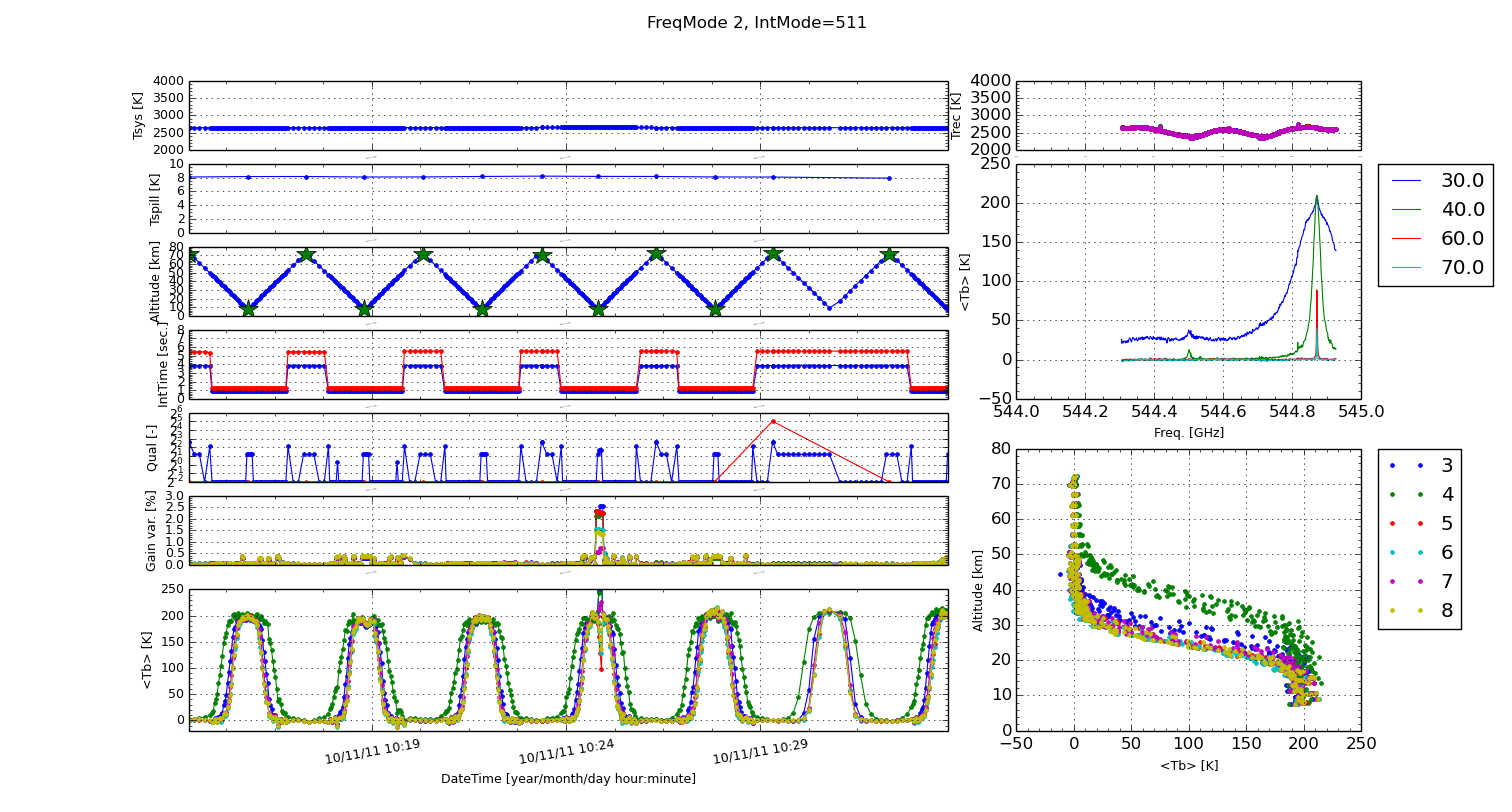
\includegraphics[width=14cm]{quality_control.png}
\caption{Quality flag example figure\lcomment{BR}{update or remove }}
\label{fig:quality}
\end{figure}

    




\chapter{Summary}


Some key issues that should be considered when examining or applying \smr\
Level1B data:
\begin{itemize}

\item \smr\ can perform observations in a number of different frequency
bands, mainly within the 486\,--\,504\,GHz and 541\,--\,581\,GHz regions.
In practise, two or three frequency bands are measured simultaneously.
For a given day, several observation modes can be applied, and hence
it is rather complicated to describe the time-sharing in a 
comprehensive way.
 

\item Calibrated spectra are expressed in terms of Rayleigh--Jeans brightness temperature.

\item \smr\ spectra contain a significant amount of broadband noise, 
due to rapid gain fluctuations, in addition to radiometric noise.

\item more to come ...\lcomment{BR}{update or remove }

\end{itemize}

